\documentclass{article}

\usepackage{paper}

\begin{document}

\setpapertitle{Convergence of Gradient Descent and Its Variants}

\setauthor[150259]{Gurpreet Singh}{guggu@iitk.ac.in}
\addauthor[150300]{Jaivardhan Kapoor}{jkapoor@iitk.ac.in}

\newcommand{\x}[1]{\vx^{#1}}
\newcommand{\xs}{\vx^{\ast}}

\newcommand{\z}[1]{\vz^{(#1)}}
\newcommand{\zs}{\vz^{\ast}}

\newcommand{\f}[2][]{\func[#1]{f}{\x{#2}}}
\newcommand{\fs}[1][]{\func[#1]{f}{\xs}}

\newcommand{\fz}[1]{f(\z{#1})}
\newcommand{\fzs}{f(\zs)}

\newcommand{\gf}[2][]{\nabla \func[#1]{f}{\x{#2}}}
\newcommand{\ggf}[1][]{\nabla \func[#1]{f}{\vx}}
\newcommand{\ggs}[1][]{\nabla \func[#1]{f}{\xs}}

\newcommand{\gfz}[1]{\nabla \fz{#1}}
\newcommand{\ggfz}{\nabla f(\vz)}

\newcommand{\fpi}[2]{\func{\Pi_{#1}}{#2}}

\renewcommand{\makeheader}{
	\begin{center}
		\parbox{0.9\textwidth}{%
			\hrule height4pt
			\vspace{5mm}

			\begin{center}
				\setstretch{1.5}
				{\fontsize{16pt}{20pt} \bt{\papertitle}}
			\end{center}

			\vspace{3mm}
			\hrule height2pt
		}

		\vspace{5mm}

		\begin{center}
			\bt{\fontsize{11}{11}\selectfont \ut{Group 10}}
		\end{center}


		\parbox{0.75\textwidth}{
			\begin{center}
				\authors
			\end{center}
		}
	\end{center}
}

\makeheader
\abstract{
	In this text, we survey prominent Gradient Descent techniques for optimization. Both, deterministic and stochastic methods are reviewed, such as SGD, Momentum, AdaGrad, ADAM and NAG. Convergence analyses of these algorithms are given, for objectives with various constraints on convexity, strong smoothness and strong convexity. Particularly for Adam, we review a recent work showing that the algorithm does not always converge, and restate the rigorous proof of the counterexample. Finally, the text aims to act as a reference for the reader to refer to convergence analyses of the above-mentioned methods, along with certain comments on the performance of these methods.
}

\begin{psection}{Introduction}

	Gradient descent is an optimization algorithm used to minimize a function by iteratively moving in the direction of steepest descent as defined by the negative of the gradient. \citep{gd-overview}. Gradient Descent was formulated by \cite{gd-original} centuries ago. Many variants of this method have arrived, since, and are used in various fields.

	Gradient Descent is predominantly used in training Deep Networks. More specifically, variants of Gradient Descent with Stochastic Update rules are used.

	This survey aims to look at various variants of Gradient Descent and analyze the convergence of each variant in simple settings.

\end{psection}

\begin{psection}{Preliminaries}

	\begin{psubsection}{Notation}

		We follow the general notation, where $\xs$ is an optimal point to be learned, \ie a local minima w.r.t. to a function, say $f : \cX \ra \bR$, where $\cX \subseteq \bR^d$ is the intersection of the domain set of $f$ and the feasible set of points. The point $\x{t}$ represents our approximation of the optimal point at a time step $t$, and the point $\hat{\vx}$ represents the optimal point as estimated by the algorithm.

		With an abuse of notation, we assume $\frac{\va}{\vM}$ to be the same as $\vM^{-1} \va$, where $\va \in \bR^d$ and $\vM \in \bR^{d \times d}$ and $\sqrt{(.)}$ or $(.)^{1/2}$ to be element-wise square root operators.

	\end{psubsection}

	\begin{psubsection}{Convex Functions}

		Convexity of a function simplifies the complexity of optimization by inducing inequalities that are helpful for convergence. Below, we define the condition for a function to be convex.
		\begin{definition}[Convex Fucntion]
			\label{def:cvx}
			A function $f: \cX \ra \bR$ is said to be convex, iff $\qforall \vx, \vy \in \cX$,
			\begin{equation}
				f(\vy)	\qge	f(\vx) + \dotp{\nabla f(\vx)}{\vy - \vx}
				\label{eq:cvx}
			\end{equation}
		\end{definition}

		If a function $f : \cX \ra \bR$ is convex, then all the following inequalities are equivalent,

		\begin{enumerate}
			\item $\qforall \vx, \vy \in \cX$
				\begin{equation*}
					f(\vy)	\qge	f(\vx) + \dotp{\nabla f(\vx)}{\vy - \vx}
				\end{equation*}
			\item $\qforall \vx, \vy \in \cX$ and $\qforall \alpha \in \brac{0, 1}$
				\begin{equation}
					\quad f(\alpha \cdot \vx + \para{1 - \alpha} \cdot \vy)	\qle	\alpha \cdot f(\vx) + \para{1 - \alpha} \cdot f(\vy)
					\label{eq:cvx-alt}
				\end{equation}
			\item If $f$ is twice differentiable, then $\qforall \vx \in \cX$
				\begin{equation}
					\nabla^2 f(\vx)	\qsucceq 0
					\label{eq:cvx-2d}
				\end{equation}
		\end{enumerate}

		Below, we define two other inequalities, Strong Convexity and Strong Smoothness, that if a function satisfies, we can prove stronger convergence bounds for that function.
		\begin{definition}[Strong Convexity]
			\label{def:sc}
			A function $f: \cX \ra \bR$ is said to be $\alpha$-SC \footnote{$\alpha$-SC ($\alpha$-SS) denotes that the function is $\alpha$-Strongly Convex ($\alpha$-Strongly Smooth)} if $\qforall \vx, \vy \in \cX$,
			\begin{equation}
				f(\vy)	\qge	f(\vx) + \dotp{\nabla f(\vx)}{\vy - \vx} + \frac{\alpha}{2} \norm{\vy - \vx}_2
				\label{eq:sc}
			\end{equation}
		\end{definition}

		\begin{definition}[Strong Smoothness]
			\label{def:ss}
			A function $f: \cX \ra \bR$ is said to be $\alpha$-SS if $\qforall \vx, \vy \in \cX$,
			\begin{equation}
				f(\vy)	\qle	f(\vx) + \dotp{\nabla f(\vx)}{\vy - \vx} + \frac{\beta}{2} \norm{\vy - \vx}_2
				\label{eq:ss}
			\end{equation}
		\end{definition}

	\end{psubsection}

	We are now equipped with the basic tools sufficient to tackle the analysis of gradient based optimization methods. We discuss some of the deterministic methods in the next section, followed by Stochastic Methods of optimization in Section 4. We then conclude with some comments on the different techniques of optimization.

\end{psection}

\begin{psection}{Deterministic Methods}

	Deterministic Methods of optimization use the actual value of the function $f$ to compute the optimization step. We will discuss this in more detail when we discuss stochastic methods of optimization. We discuss three such methods of optimization, Vanilla Gradient Descent, Momentum and Nesterov's Accelerated Gradient Method and discuss their convergence under certain conditions.

	The convergence of an algorithm is measured using the regret of the algorithm, which is defined, for a data point $\vx$ as
	\begin{align*}
		\rgrt{\vx} \qdeq f(\vx) - f(\xs)
	\end{align*}
	Therefore, our objective, when we are showing the convergence of an method is bound the regret of that function.

	The algorithm for Vanilla Gradient Descent is given in Algorithm \hyperlink{algo:1}{1}. Most descent algorithms follow the same rules, with minor additions and improvements to the optimization (update) step. The function $h$ determines the form of the output, for example, $h$ can be an average function, \ie $h(\x{1} \dots \x{T}) = \frac{1}{T} \sum_{t = 1}^T \vx^t$, or we can simply set $h$ to return the last time step's estimate, \ie $h(\x{1} \dots \x{T}) = \x{T}$.

	\begin{algo}[0.9\textwidth]{Deterministic Gradient Descent}

		\bt{Input:} \quad Step sizes $\set{\eta_t > 0}_{t = 1}^T$ and a function $h : \cS \mapsto \cX $ where $\cS$ is a sequence of data points. \sbr

		\bt{Output:}\, $\hat{\vx} \in \cH$, where $\hat{\vx} = \func{h}{\vx^{(1)} \dots \vx^{(T)}}$ \sbr

		\bt{Steps:}

		\begin{enumerate}
			\item Initialize $\x{0} \in \cH$
			\item For $t = 1 \dots T$, do
				\begin{align}
					\vg_t		&\eq	\gf{t}							\tag{Gradient Step}		\\
					\x{t + 1}	&\eq	\x{t} - \alpha_t \cdot \vg_t	\tag{Optimization Step}
				\end{align}
			\item Return $\hat{\vx} = \func{h}{\x{1} \dots \x{T}}$
		\end{enumerate}

	\end{algo}

	\begin{psubsection}{Gradient Descent}

		Vanilla Gradient Descent iteratively solves the optimization problem, using the gradient of the function $f$ at a time step. The idea is to update the parameter $\vx$ in the opposite direction of the gradient of the optimization objective.

		The projection step ensures that the predictions remain within the feasible set of points, \ie $\vX$.

		In case of Vanilla Gradient Descent, the values of $\set{\alpha_t}_{t = 1}^T$ are kept to be equal to the step sizes. Therefore, the update step can be written as
		\begin{align}
			\x{t+1}	\eq	\x{t} - \eta_t \cdot \gf{t}
			\tag{\st{Vanilla GD}}
			\label{eq:vgd}
		\end{align}

		In the follow subsections, we discuss the convergence and the necessary conditions required for this convergence for different settings for the optimizer function $f$.

		\begin{note}
			For the rest of the article, we use $\Phi_t$ to denote the difference between the $t$\tth estimate of the optimal point and the real optimal value, \ie $\f{t} - \fs$ and $\sD_t$ to denote the difference between the current point estimate and the optimal point, \ie $\norm{\x{t} - \xs}_2$. $\vPhi_t$ is known as the Lyapunov function which basically defines the potential at a time step.
		\end{note}

		The convergence analysis were borrowed from the analysis discussed in the class of CS777, IITK \cite{gd}.

		\begin{pssubsection}{When $f$ is Convex with Bounded Gradients}

			First, we state the result, and later we give the derivation for the result.

			\begin{theorem}
				If $f : \vX \to \bR$ is convex and $\qforall \vx \in \cX, \ggf$ exists, then for bounded gradients, we say
				\begin{align}
					\frac{1}{T} \sum_{t = 0}^T \vPhi_t \qle \frac{1}{2\sqrt{T}}\sD_0 \cdot \sG
					\label{eq:gd-cvx-bddg}
				\end{align}
				\label{th:gd-cvx-bddg}

				\begin{proof}
					From the convexity (equation \ref{eq:cvx}) of the function $f$, we have
					\begin{align*}
						\Phi_t	&\qle	\dotp{\gf{t}}{\x{t} - \xs} \\
						&\eq	\frac{1}{\eta} \dotp{\eta \cdot \gf{t}}{\x{t} - \xs}
					\end{align*}

					Here, we mention two properties, which will be used here, as well as a few times in later proofs

					\begin{property}
						For any two vectors $\va, \vb \in \bR^m$,
						\begin{equation}
							\norm{\va + \vb}_2^2 - \norm{\va}_2^2 - \norm{b}_2^2	\eq[a]	2\dotp{a}{b}	\eq[b]	\norm{\va}_2^2 + \norm{b}_2^2 - \norm{\va - \vb}_2^2
							\label{eq:dotp}
						\end{equation}
					\end{property}

					Using property \hyperref[eq:dotp]{\ref*{eq:dotp}a}, we can write the above inequality as
					\begin{align*}
						\Phi_t	&\qle	\frac{1}{2 \eta} \para{\norm{\x{t} - \xs}_2^2 + \eta^2 \norm{\gf{t}}_2^2 - \norm{\x{t} - \eta \cdot \gf{t} - \xs}} \\
						&\qle	\frac{1}{2 \eta} \para{\sD_t^2 + \eta^2 \sG^2 - \sD_{t + 1}^2} \\
						&\eq	\frac{1}{2 \eta} \para{\sD_t^2 - \sD_{t + 1}^2} + \frac{\eta}{2} \sG^2
					\end{align*}

					Adding for $t = 0 \dots T$, we get
					\begin{align*}
						\sum_{t = 0}^T	\Phi_t						&\qle	\frac{1}{2 \eta} \para{\sD_0^2 - \sD_{T+1}^2} + \frac{\eta\,T}{2} \cdot \sG^2 \\
						\implies \frac{1}{T} \sum_{t = 0}^T	\Phi_t	&\qle	\frac{1}{2 \eta \, T} \sD_0^2 + \frac{\eta}{2} \cdot \sG^2
					\end{align*}

					Since this inequality is true for any choice of $\eta$, we can minimize the RHS with respect to $\eta$ to get an even stronger bound.

					Therefore, we get
					\begin{align*}
						\frac{1}{T} \sum_{t = 0}^T \vPhi_t \qle \frac{1}{2 \sqrt{T}}\sD_0 \cdot \sG
					\end{align*}

					This proves theorem \ref{th:gd-cvx-bddg}
				\end{proof}
			\end{theorem}

			However, how does the above inequality ensure that gradient descent actually gives us a good estimate of the optimal point $\xs$? This can, in fact, be seen as another result of convexity in the function, since, using the convexity properties of $f$, we can claim
			\begin{align*}
				\func{f}{\hat{\vx}} \eq \func{f}{\frac{1}{T} \sum_{t = 1}^T \x{t}}	\qle	\frac{1}{2\sqrt{T}} \sD_0^2 \sG^2 + \func{f}{\xs}
			\end{align*}

			Therefore, substituting this in equation \ref{eq:gd-cvx-bddg}, we can write
			\begin{equation}
				\rgrt{\hat{\vx}} \eq \func{f}{\hat{\vx}} - \fs	\qle	\frac{1}{2\sqrt{T}} \sD_0^2 \sG^2
				\label{eq:gd-1-bound}
			\end{equation}

			Hence for a case when the function $f$ is convex and has bounded gradients, we can say that our regret is bounded with an order of $\bigO{\frac{1}{\sqrt{T}}}$, given the return function, \ie $h$ is an averaging function.

		\end{pssubsection}

		\begin{pssubsection}{When $f$ is Convex and $\vbeta$-Strongly Smooth}

			We now look at a more restrictive setting, in the sense that this setting allows us to have a much stronger bound than the bound given in equation \ref{eq:gd-1-bound}. Again, we state the result first, then give a convergence proof for the same. \sbr

			\begin{theorem}
				If $f : \vX \to \bR$ is convex, $\beta$-smooth and $\qforall x$, $\gf{t}$ exists, we can say
				\begin{align}
					\frac{1}{T} \sum_{t = 0}^T \Phi_t	\qle	\frac{1}{2 \eta} \cdot \frac{\sD_0^2}{T}
					\label{eq:gd-cvx-bsm}
				\end{align}
				\label{th:gd-cvx-bsm}

				\begin{proof}
					From the convexity and smoothness of the function $f$, we have, respectively
					\begin{align}
						\fs			&\qge	\f{t} - \dotp{\gf{t}}{\x{t} - \xs} \label{eq:gd2-beta} \\
						\f{t + 1}	&\qle	\f{t} + \dotp{\gf{t}}{\x{t + 1} - \x{t}} + \frac{\beta}{2} \norm{\x{t + 1} - \x{t}}_2^2 \nonumber
					\end{align}

					From the update equation of Gradient Descent, we can replace $\x{t + 1}$ with $\x{t} - \eta_t \cdot \gf{t}$. Therefore, we get
					\begin{align}
						\f{t + 1}	&\qle	\f{t} + \para{\frac{\beta}{2} - \frac{1}{\eta_t}} \norm{\eta_t \cdot \gf{t}}_2^2 \label{eq:gd2-cvx}
					\end{align}

					Subtracting equation \ref{eq:gd2-beta} from \ref{eq:gd2-cvx}, we get
					\begin{align*}
						\Phi_{t + 1}	&\qle	\para{\frac{\beta}{2} - \frac{1}{\eta_t}} \norm{\eta_t \cdot \gf{t}}_2^2 - \dotp{\gf{t}}{\x{t} - \xs} \\
						&\eq	\para{\frac{\beta}{2} - \frac{1}{\eta_t}} \norm{\eta_t \cdot \gf{t}}_2^2 - \frac{1}{\eta_t} \dotp{\eta_t \cdot \gf{t}}{\x{t} - \xs}
					\end{align*}

					Using property \hyperref[eq:dotp]{\ref*{eq:dotp}a}, we can write this, similarly to the previous case, as
					\begin{align*}
						\Phi_{t + 1}	&\qle	\para{\frac{\beta}{2} - \frac{1}{\eta_t}} \norm{\eta_t \cdot \gf{t}}_2^2 + \frac{1}{2 \eta_t} \para{\sD_t^2 + \norm{\eta_t \cdot \gf{t}}_2^2 - \sD_{t + 1}^2} \\
						\Phi_{t + 1}	&\qle	\frac{1}{2 \eta_t} \para{\sD_t^2 - \sD_{t + 1}^2} + \para{\frac{\beta}{2} - \frac{1}{2 \eta_t}} \norm{\eta_t \cdot \gf{t}}_2^2
					\end{align*}

					Suppose if we set $\eta_t \le \frac{1}{\beta}$, then the second term is always positive. Hence, we can write
					\begin{align*}
						\Phi_t	\qle	\frac{1}{2 \eta_t} \para{\sD_t^2 - \sD_{t + 1}^2}
					\end{align*}

					Adding for $t = 0 \dots T$, we get
					\begin{align*}
						\sum_{t = 0}^T	\Phi_t						&\qle	\frac{1}{2 \eta_t} \para{\sD_0^2 - \sD_{T + 1}^2} \\
						\implies \frac{1}{T} \sum_{t = 0}^T	\Phi_t	&\qle	\frac{1}{2 \eta} \frac{\sD_0^2}{T}
					\end{align*}

					This completes the proof.
				\end{proof}
			\end{theorem}

			Therefore, we can see that this bound offers much more than the bound in the previous case, as we can see that for large values of $T$, the bound will tend towards 0, and hence we can be sure our estimate of $\fs$ is good.

			Also, similar to the previous case, we can write, using the properties of convexity,
			\begin{align*}
				\func{f}{\hat{\vx}} \eq \func{f}{\frac{1}{T} \sum_{t = 1}^T \x{t}}	\qle	\frac{1}{2 \eta} \cdot \frac{\sD_0^2}{T} + \func{f}{\xs}
			\end{align*}
			\begin{equation}
				\implies \rgrt{\hat{\vx}}	\qle	\frac{1}{2 \eta} \cdot \frac{\sD_0^2}{T}
				\label{eq:gd-2-bound}
			\end{equation}

			\begin{remark}
				In this case, setting $\eta = \frac{1}{\beta}$ would result in the most optimal bound.
			\end{remark}

			\begin{remark}
				The bound in this case is $\bigO{\frac{1}{T}}$ and therefore the convergence will be much faster and better in this case as opposed to simply convex case with bounded gradients.
			\end{remark}

		\end{pssubsection}

	\end{psubsection}

	\begin{psubsection}{Momentum}

		The gradient descent algorithm described above exhibits good convergence properties for "nice" functions (having smoothness and convexity/strong convexity properties). However, for poorly scaled objectives, for which in each dimension, the objective changes very differently, Gradient Descent may converge very slowly. This is because sometimes the updates get trapped in narrow valleys, where the direction of steepest descent for a given rate parameter causes the updates to oscillate between two sides of the smaller axis of the valley, and correspondingly move very slowly through the larger axis of the valley. \cite{gd-overview}

		A solution devised for this problem was inspired from a physical analogy of a ball rolling down a hill. The ball has some momentum associated with it, and thus on the basis of this virtue, it can move past small bumps (local minima) and narrow valleys (poorly scaled regions). It takes into account a convex combination of the current and previous updates, ain to giving the updates a short-term memory. An additional parameter $\beta$ is added to the GD updates to account for this momentum term, and correspondingly the updates become
		\begin{align*}
			\vz^{t+1} &\eq \beta \cdot \vx^t+\nabla f(\vx^t) \\
			\vx^{t+1} &\eq \vx^t-\alpha \cdot \vz^{t+1}
		\end{align*}
		which amounts to
		\begin{equation}
			\vx^{t+1} \eq \vx^t-\alpha\nabla f(\vx^t) + \beta(\vx^t-\vx^{t-1})
			\tag{\st{Momentum}}
		\end{equation}

		The convergence rate of this method compared with the above method shows that the \textit{condition number}, denoted by $\kappa=\frac{\beta}{\alpha}$, plays a large role in the speedup obtained using momentum. The gradient descent method, $\alpha$-s.c. and $\beta$-s.s convex function gives the following result
		\begin{align*}
			\norm{\vx^t-\vx^*} \eq \frac{\kappa-1}{\kappa+1}\norm{\vx^0-\vx^*}
		\end{align*}

		However, using momentum yields us the following result:
		\begin{align*}
			\norm{\vx^t-\vx^*} \eq \frac{\sqrt{\kappa}-1}{\sqrt{\kappa}+1}\norm{\vx^0-\vx^*}
		\end{align*}

		This means for a sufficient large $\kappa=100$ the optimum is reached 10 times faster.

		We consider a convex $f$ which is $\beta$-strongly smooth, and derive the convergence rate for the Lyapunov function, $\Phi_t=f(\vx^t)-f(\vx^*)$.

		\begin{theorem}
			\label{th:momentum}
			If $f$ is convex and $L$-SS, then the above updates satisfy, for learning rate $\alpha$ an momentum parameter $\beta$,
			\begin{equation}
				\rgrt{\hat{\vx}} \eq \func{f}{\hat{\vx}} - \fs	\qle	\frac{1}{T} \para{2 \beta F +\frac{1-\beta}{2\alpha}\sD_0^2}
				\label{eq:momentum}
			\end{equation}
			That is, the error scale down inversely with the number of time steps.
			\begin{proof}
			We assume $\beta\in[]0,1)$. Also, define:

			\begin{equation*}
				\vp_t \eq \frac{\beta}{1-\beta}(\vx^t-\vx^{t-1})    
			\end{equation*}
			from which we have
			\begin{equation*}
				\vx^{t+1}+\vp{t+1} \eq \vx^t+\vp^t-\frac{\alpha}{1-\beta}\nabla f(\vx^t)    
			\end{equation*}

			Consider

			\begin{align*}
				\norm{\vx^{t+1}+\vp^{t+1}-\vx^*}^2 &\eq \norm{\vx^{t}+\vp^{t}-\vx^*}^2-\frac{2\alpha}{1-\beta}\cdot\langle\vx^{t}+\vp^{t}-\vx^*,\nabla f(\vx^t)\rangle + \para{\frac{\alpha}{1-\beta}}^2\norm{\nabla f(\vx^t)}^2\\
				&\eq \norm{\vx^{t}+\vp^{t}-\vx^*}^2-\frac{2\alpha}{1-\beta} \cdot \langle\vx^{t}-\vx^*,\nabla f(\vx^t)\rangle -\frac{2\alpha\beta}{(1-\beta)^2}\langle\vx^{t}-\vx^{t-1},\nabla f(\vx^t)\rangle\\ &\quad+\quad \para{\frac{\alpha}{1-\beta}}^2\norm{\nabla f(\vx^t)}^2
			\end{align*}

			From the strongly smooth property, it follows that:

			\begin{equation}
				\norm{\nabla f(\vx^t)}^2 \qle L\langle\vx^{t}-\vx^{t-1},\nabla f(\vx^t)\rangle\\
				f(\vx^t) - f(\vx^*) + \frac{1}{2L}\norm{\nabla f(\vx^t)}^2 \qle \langle\vx^{t}-\vx^{t-1},\nabla f(\vx^t)\rangle
			\end{equation}

			Using these inequalities, we get

			\begin{align*}
				\norm{\vx^{t+1}+\vp^{t+1}-\vx^*}^2 &\eq \norm{\vx^{t}+\vp^{t}-\vx^*}^2-\frac{2\alpha}{1-\beta}(f(\vx^t) - f(\vx^*) + \frac{1}{2L}\norm{\nabla f(\vx^t)}^2) \\
				&\quad-\quad \frac{2\alpha}{1-\beta}\langle\vx^{t} -\vx^*,\nabla f(\vx^t)\rangle + \para{\frac{\alpha}{1-\beta}}^2\norm{\nabla f(\vx^t)}^2
			\end{align*}

			Applying convexity to the inner product, we obtain

			\begin{align*}
				\norm{\vx^{t+1}+\vp^{t+1}-\vx^*}^2 &\eq \norm{\vx^{t}+\vp^{t}-\vx^*}^2-\frac{2\alpha}{1-\beta}(f(\vx^t) - f(\vx^*) + \frac{1}{2L}\norm{\nabla f(\vx^t)}^2) \\
				&\quad-\quad\frac{2\alpha}{1-\beta}(f(\vx^t)-f(\vx^{t-1}))+\para{\frac{\alpha}{1-\beta}}^2\norm{\nabla f(\vx^t)}^2
			\end{align*}

			Now subtract $\frac{2\alpha\beta}{(1-\beta)^2}f(\vx^*)$ from both sides and collect the terms to obtain

			\begin{align*}
				\para{\frac{2\alpha}{1-\beta}+\frac{\alpha\beta}{(1-\beta)^2}}(f(\vx^t)-f(\vx^*)) +\norm{\vx^{t+1}+\vp^{t+1}-\vx^*}^2 &\qle \frac{2\alpha\beta}{(1-\beta)^2}(f(\vx^{t-1})-f(\vx^*)) \\
				&\quad+\quad\norm{\vx^{t}+\vp^{t}-\vx^*}^2\\
				&\quad+\quad\para{\frac{\alpha}{1-\beta}}\para{\frac{\alpha}{1-\beta}-\frac{1}{L}}\norm{\nabla f(\vx^t)}^2
			\end{align*}

			For $\alpha\in(0,(1-\beta)/L]$, we take $\alpha=(1-\beta)/L$, so that the last term vanishes to give

			\begin{align*}
				\para{\frac{2\alpha}{1-\beta}+\frac{\alpha\beta}{(1-\beta)^2}}(f(\vx^t)-f(\vx^*)) +\norm{\vx^{t+1}+\vp^{t+1}-\vx^*}^2 &\qle \frac{2\alpha\beta}{(1-\beta)^2}(f(\vx^{t-1})-f(\vx^*)) \\
				&\quad+\quad \norm{\vx^{t}+\vp^{t}-\vx^*}^2
			\end{align*}

			Sum over both sides, to get
			\begin{align*}
				\para{\frac{2\alpha}{1-\beta}}\sum_{t=1}^{T}\Phi_t\qle\para{\frac{2\alpha\beta}{(1-\beta)^2}}\Phi_1 + \norm{\vx^1-\vx^*}^2
			\end{align*}
			This gives us our required inequality.
		\end{proof}
	\end{theorem}

	From the bound above, we can see that the function $h$ will be an averaging function in this case as well, and we can find the regret bound for this case similarly. Also, in this case, the regret bound will be $\bigO{\frac{1}{T}}$.

\end{psubsection}

\begin{psubsection}{Nesterov's Accelerated Gradient}

	NAG also takes advantage of the momentum term in the update equations, however the updates are made smarter to slow down when close to an optima. NAG obtains this by adding a lookahead term in the update equations. Figure \ref{fig:nag-vs-mom} below roughly describes the difference between the updates. Notice that the update in NAG first applies the momentum term, and then at the new position, applies the corrective gradient update.

	\begin{figure}[h]
		\centering
		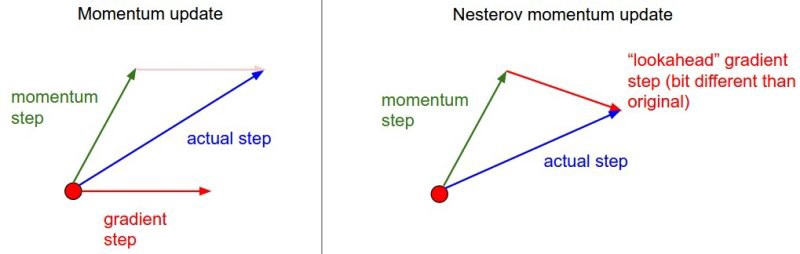
\includegraphics[width=0.6\textwidth]{includes/nag-vs-mom.jpeg}
		\caption{A look on updates for Momentum and NAG \quad (\et{Source: Stanford CS231n Class})}
		\label{fig:nag-vs-mom}
	\end{figure}

	For NAG, we consider the case where $f$ is convex and $\beta$-SS.

	\begin{theorem}
		\label{th:nag}
		If $f$ is convex and $\beta$-SS, then Nesterov Accelerated Gradient satisfies
		\begin{equation}
			\f{T} - \fs	\qle	\frac{2 \beta \sD_0^2}{(T - 1)^2}
			\label{eq:nag}
		\end{equation}

		\begin{proof}
			From the $\beta$-Smoothness of the function $f$, we have
			\begin{align}
				\f{t+1}	&\qle	\fz{t} + \dotp{\gfz{t}}{\x{t+1} - \z{t}} + \frac{\beta}{2} \norm{\x{t+1} - \z{t}}_2^2 \nonumber \\
				\implies \f{t+1}	&\qle	\fz{t} + \para{\frac{\beta}{2} - \frac{1}{\eta}} \norm{\x{t + 1} - \z{t}}_2^2 \label{eq:nag-beta-bound}
			\end{align}

			Using the convexity of function $f$, we can write
			\begin{align}
				f(\vx)	&\qge	\fz{t} + \dotp{\gfz{t}}{\vx - \z{t}} \nonumber \\
				\implies f(\vx)	&\qge	\fz{t} + \frac{1}{\eta} \dotp{\x{t+1} - \z{t}}{\vx - \z{t}} \label{eq:nag-cvx-bound}
			\end{align}

			using equations \ref{eq:nag-beta-bound} and \ref{eq:nag-cvx-bound}, we can say
			\begin{align}
				\f{t + 1} - f(\vx)	\qle	\para{\frac{\beta}{2} - \frac{1}{\eta}} \norm{\x{t + 1} - \z{t}}_2^2 - \frac{1}{\eta} \dotp{\x{t+1} - \z{t}}{\vx - \z{t}}
				\label{eq:nag-diff-bound}
			\end{align}

			We can now move on to find a bound similar to given in the theorem. First, note
			\begin{align*}
				\lambda_t^2 \cdot \Phi_{t + 1} - \lambda_{t - 1}^2 \cdot \Phi_{t}	&\eq	\lambda_t \cdot \para{\lambda_t \cdot \Phi_{t + 1} - \para{\lambda_t - 1} \cdot \Phi_t} \\
				&\eq	\lambda_t \cdot \para{\f{t + 1} - \fs} + \lambda_t \cdot \para{\lambda_t - 1} \para{\f{t + 1} - \f{t}}
			\end{align*}
			Since $\qforall t > 0$, $\lambda_t > 1$, using equation \ref{eq:nag-diff-bound}, we can derive the following inequality
			\begin{align*}
				\lambda_t^2 \cdot \Phi_{t + 1} - \lambda_{t - 1}^2 \cdot \Phi_{t}	&\qle	\lambda_t^2 \cdot \para{\frac{\beta}{2} - \frac{1}{\eta}} \norm{\x{t + 1} - \z{t}}_2^2 \ + \\
				&\hspace{2cm} + \ \frac{\lambda_t}{\eta} \cdot \dotp{\x{t+1} - \z{t}}{\xs + \para{\lambda_t - 1} \cdot \x{t} - \lambda_t \cdot \z{t}}
			\end{align*}

			Now, suppose we fix $\eta = 1 / \beta$. Therefore, we can rewrite the above inequality as
			\begin{align*}
				\lambda_t^2 \cdot \Phi_{t + 1} - \lambda_{t - 1}^2 \cdot \Phi_{t}	&\qle	- \frac{\beta}{2} \cdot \bigg( \norm{\lambda_t \cdot \para{\x{t + 1} - \z{t}}}_2^2 \ - \\
				&\hspace{2cm} - \ 2 \dotp{\lambda_t \cdot \para{\x{t+1} - \z{t}}}{\xs + \para{\lambda_t - 1} \cdot \x{t} - \lambda_t \cdot \z{t}} \bigg)
			\end{align*}

			From property \hyperref[eq:dotp]{\ref*{eq:dotp}b}, where $\va = \lambda_t \cdot \para{\x{t + 1} - \z{t}}$ and $b = \xs + \para{\lambda_t - 1} \cdot \x{t} - \lambda_t \cdot \z{t}$, we can write this as
			\begin{align}
				\lambda_t^2 \cdot \Phi_{t + 1} - \lambda_{t - 1}^2 \cdot \Phi_{t}	&\qle	- \frac{\beta}{2} \cdot \bigg( \norm{\lambda_t \cdot \x{t + 1} - \para{\lambda_t - 1} \cdot \x{t} - \xs}_2^2 \ - \nonumber \\
				&\hspace{3cm} - \ \norm{\lambda_t \cdot \z{t} - \para{\lambda_t - 1} \cdot \x{t} - \xs} \bigg)_2^2
				\label{eq:nag-diff}
			\end{align}

			Now, from the definition of $\z{t + 1}$, we can write
			\begin{align}
				\z{t + 1}	&\eq	\x{t + 1} + \gamma_t \cdot \para{\x{t} - \x{t + 1}} \nonumber \\
				\implies \lambda_{t + 1} \cdot \z{t + 1}	&\eq	\lambda_{t + 1} \cdot \x{t + 1} + \para{1 - \lambda_t} \cdot \para{\x{t } - \x{t + 1}} \nonumber \\
				\implies \lambda_{t + 1} \cdot \z{t + 1} - \para{\lambda_{t + 1} - 1} \cdot \x{t + 1}	&\eq	\lambda_t \cdot \x{t + 1} - \para{\lambda_t - 1} \cdot \x{t} \label{eq:nag-us}
			\end{align}

			We can substitute the term in equation \ref{eq:nag-diff} using equation \ref{eq:nag-us}. Now, define $\vu_t = \lambda_t \cdot \z{t} - \para{\lambda_t - 1} \cdot \x{t} - \xs$. Therefore, we can write
			\begin{align*}
				\lambda_t^2 \cdot \Phi_{t + 1} - \lambda_{t - 1}^2 \cdot \Phi_{t}	\qle	\frac{\beta}{2} \cdot \para{\norm{\vu_t}_2^2 - \norm{\vu_{t + 1}}_2^2}
			\end{align*}

			Adding this from $t = 0, 1 \dots (T - 1)$
			\begin{align*}
				\lambda_{T - 1}^2 \Phi_{T}	&\qle	\frac{\beta}{2} \cdot \para{\norm{\vu_0}_2^2 - \norm{\vu_T}_2^2} + \lambda_{0}^2 \cdot \Phi_{0}	\qle	\frac{\beta}{2} \cdot \norm{\vu_0}_2^2 + \lambda_0^2 \cdot \Phi_0
			\end{align*}

			We know $\lambda_0 = 0$. Also, using induction, it is easy to see that $\qforall t \ge 2$, $\lambda_{t} > t / 2$. therefore, we have
			\begin{align*}
				\Phi_T	\qle	\frac{2 \beta \cdot \norm{\vu_0}_2^2}{(T - 1)^2}	\eq	\frac{2 \beta \cdot \sD_0^2}{(T - 1)^2}
			\end{align*}
		\end{proof}
	\end{theorem}

	From the bound given above, we can see that the function $h$ simply returns the value from the last iteration. Also, the bound in this case is much stronger, with $\bigO{\frac{1}{T^2}}$.

\end{psubsection}

\end{psection}

\begin{psection}{Stochastic Optimization}

	Deterministic methods, although guaranteeing convergence, can be slow and each time step can be expensive to perform. However, most convex functions can be written as a sum of simpler convex optimization objectives. In such a case, optimization can be made more effective by taking gradient steps with respect to each subfunction. Such an optimization technique is termed as Stochastic Optimization.

	Logistic Regression with mini-batch learning can be seen as a simple example for Stochastic Optimization. The generic adaptive method for Stochastic Optimization is given in \hyperlink{algo:2}{Algorithm 2}, however we still do not give the forms of the functions $\set{\phi_t, \psi_t}_{t = 1}^T$, which vary depending on different algorithms.

	Stochastic Optimization has a natural annealing property which makes then suitable for even non-convex optimization, however a theoretical convergence guarantee cannot be formulate in that case.

	\begin{algo}[0.9\textwidth]{Generic Adaptive Method}

		\bt{Input:} \quad step sizes $\set{\eta_t \in \bR^{+}}_{t = 1}^T$, a sequence of functions $\set{\phi_t, \psi_t}_{t = 1}^T$, and a sequence of convex sub-objectives $\set{f_t}_{t = 1}^T$ \sbr

		\bt{Output:}\, $\hat{\vx} \in \cH$, where $\hat{\vx} = \func{h}{\vx^{(1)} \dots \vx^{(T)}}$ \sbr

		\bt{Steps:}

		\begin{enumerate}
			\item Initialize $\vx^{(0)} \in \cH$
			\item For $t = 1 \dots T$, do
				\begin{align*}
					\vg_t			&\eq	\gf[t]{t}					\\
					\vm_t			&\eq	\func{\phi_t}{\vg_1 \dots \vg_t}			\\
					V_t				&\eq	\func{\psi_t}{\vg_1 \dots \vg_t}			\\
					\vx^{(t + 1)}	&\eq	\vx^{(t)} - \eta_t V_t^{- 1 / 2} \vm_t
					%\vx^{(t)}		&\eq	\func{\Pi_{\cH, V^{1/2}}}{\vz^{(t + 1)}}
				\end{align*}
			\item Return $\hat{\vx} = \func{h}{\vx^{(1)} \dots \vx^{(T)}}$
		\end{enumerate}

	\end{algo}

	\begin{psubsection}{Stochastic Gradient Descent}

		Parts of this section is borrowed from \cite{sgd}. In cases of large amount of data, the objective function that has to be calculated and correspondingly its gradient for the update steps in optimization procedures scale linearly with the data. Thus, sometimes the subset of data is chosen and gradients are calculated according to that subset of data. SGD is restricted to optimizations of these types, where the data parameters control the value of the function, and the data is assumed to be sampled from an unknown data distribution, $\cD$.

		Let us denote the parameter of choosing as $\vtheta \sim \cD$. Then the function is of the form $f(\vx; \vtheta)$, such that
		\begin{align*}
			f(\vx)=\E[\theta\sim\cD]{f(\vx; \vtheta)}
		\end{align*}

		Therefore, we can choose our sub-functions to be of the form
		\begin{align*}
			f_t(\vx) \qdeq f(\vx; \vtheta_t)
		\end{align*}
		where $\vtheta_t \sim \cD$ is an arbitrary value sampled from the data distribution i.i.d.

		In the update equations for SGD, we assume $\phi_t$ to return the last gradient, and $\psi_t$ to return $\vI$. More formally, SGD follows the update equations from Algorithm \hyperlink{algo:2}{2}.
		\begin{equation}
			\func{\phi_t}{\vg_1 \dots \vg_t} \eq \vg_t \quad\text{and}\quad	\func{\psi_t}{\vg_1 \dots \vg_t} \eq \vI
			\tag{\st{SGD}}
		\end{equation}

		Also, since the data points ($\vtheta_t$) are assumed to be i.i.d, we can say the following about the gradients $\vg_t$
		\begin{align*}
			\E{\vg_t \pipe \cH_t} \eq \nabla f(\vx)
		\end{align*}
		where $\cH_t$ is the history of $\vg_t$, $\cH_t = \set{\vg_1,\vg_2 \dots \vg_{t-1}}$. The above equation is satisfied as
		\begin{align*}
			\E{\vg_t(\vx)} \eq \E[\theta]{\nabla f(\vx,\theta)} \eq \nabla \E[\theta]{(\vx,\theta)} \eq \nabla f(\vx)
		\end{align*}

		The convergence analysis of the above algorithm is presented for convex $f$ with bounded gradients. It is also assumed that $\cC$ is convex. Another assumption we make is that $f(\vx,\theta)$ is convex for all $\theta$. Also, $\norm{\vg_t}_2<G$.

		Using convexity condition between $\vx^t$ and $\vx^*$, where the latter is the optimum, we get
		\begin{equation*}
			\begin{split}
				f(\vx^t)-f(\vx^*) &\qle \langle\nabla f(\vx^t),\vx^t-\vx^*\rangle \\
			\end{split}
		\end{equation*}
		This is not particularly useful to us, since the algorithm deals with $\vg_t$ instead of $\nabla f(\vx^t)$. Therefore we work with $f(\vx,\theta)$ and $\vg_t$, and then take expectation over $\delta$ on both sides. This will get rid of $\theta$.
		\begin{equation*}
			\begin{aligned}
				f(\vx^t,\theta^t)-f(\vx^*,\theta^t) &\qle \langle\vg_t,\vx^t-\vx^*\rangle
			\end{aligned}
		\end{equation*}
		We now take expectation ($\E{\cdot\vert\cH_t}$) on both sides:
		\begin{equation*}
			\begin{aligned}
				f(\vx^t)-f(\vx^*) &\qle \langle\vg_t,\vx^t-\vx^*\rangle \\
				&\qle \eta \frac{G^2}{2} + \frac{D_t^2}{2\eta}-\frac{\norm{\vz^{t+1}-\vx^*}_2^2}{2\eta}\\
				&\qle \eta \frac{G^2}{2} + \frac{D_t^2}{2\eta}-\frac{D_{t_1}^2}{2\eta}
			\end{aligned}
		\end{equation*}
		We now take the expectation w.r.t $\cH_t$ on both the sides, and sum over all $t$. The term $D_t^2-D_{t+1}^2$ telescopes, giving the following result for $\eta=\frac{D_0}{G\sqrt{T}}$:
		\begin{equation*}
			\begin{aligned}
				\frac{1}{T}\E[\cH_t]{f(\vx^t)}\qle f(\vx^*) + \frac{2G^2D_0^2}{\sqrt{T}}
			\end{aligned}
		\end{equation*}
		Since the procedure is stochastic, we need a Chernoff-like bound for the convergence of $f(\vx^t)$- $f(\vx^*)$. For this, we propose 3 claims, for which the proof can be referred to in the cited article:

		\begin{claim}
			With high probability($1-\delta$),
			$$
			\sum(f(\vx^t)-f(\vx^t,\theta^t))\qle \sqrt{T}log(\frac{1}{\delta})
			$$
		\end{claim}

		\begin{claim}
			With high probability($1-\delta$),
			$$
			\sum(f(\vx^*,\theta^t)-f(\vx^*))\qle \sqrt{T}log(\frac{1}{\delta})
			$$
		\end{claim}
		\begin{claim}
			With high probability($1-\delta$),
			$$
			\sum(f(\vx^t,\theta^t)-f(\vx^*,\theta^t))\qle \sqrt{T}log(\frac{1}{\delta})
			$$
		\end{claim}
		Combining the above 3 inequalities together, we get, w.h.p($1-\delta$)
		\begin{equation*}
			\begin{aligned}
				\frac{1}{T}\sum(f(\vx^t)-f(\vx^*)) \qle \frac{1}{\sqrt{T}}log(\frac{3}{\delta})
			\end{aligned}
		\end{equation*}
		which gives us a confidence bound on the convergence of the function to its optimum.
	\end{psubsection}

	\begin{psubsection}{Adam}
		In case of Adam (and AdaGrad, later), we define the regret to be with respect to each subfunction, and therefore the total regret is written as
		\begin{equation}
			R(T) \qdeq \sum_{t = 1}^T f_t(\hat{\vx^t}) - f_t(\xs)
			\label{eq:adam-regret}
		\end{equation}
		This is because all operations are done pointwise, and therefore the expected values of the gradients is difficult to compute.

		Adam, short for Adaptive Moment Estimation, given by \cite{adam}, is an Adaptive Method and a variant of AdaGrad, which gives Exponentially Moving Averages. The key idea is to use exponentially moving average as function $\psi_t$ instead of the simple averaging function we have seen until now.

		Although other popular Adaptive Methods based on Exponentially Moving Averages exist, such as RMSprop, Nadam and AdaDelta, we only discuss Adam and its convergence in this article.

		The update step for Adam is given as below
		\begin{equation}
			\tag{\st{Adam}}
			\begin{split}
				\func{\phi_t}{\vg_1 \dots \vg_t} &\eq \beta_1 \cdot \func{\phi_{t - 1}}{\vg_1 \dots \vg_{t - 1}} + (1 - \beta_1) \cdot \vg_t \\
				\func{\psi_t}{\vg_1 \dots \vg_t} &\eq \beta_2 \cdot \func{\psi_{t - 1}}{\vg_1 \dots \vg_{t - 1}} + (1 - \beta_2) \cdot \tfunc{diag}{\vg_t^2}
			\end{split}
			\label{eq:adam}
		\end{equation}

		There is an additional initial bias correction step \citep[see][]{adam}, where we write
		\begin{align*}
			\widehat{\vm}_t	\eq \frac{\vm_t}{1 - \beta_1^t} \quad\text{and}\quad \widehat{\vV}_t \eq \frac{\vV_t}{1 - \beta_2^t}
		\end{align*}
		and use these instead of $\vm_t$ and $\vV_t$ in the update step.

		\begin{pssubsection}{Convergence Analysis of Adam}

			We give the same convergence analysis as given by \cite{adam}, but there are a few mistakes in the convergence analysis provided by them. We tackle these mistakes and try to give a better proof. As was previously done, we first state the regret bound and the assumptions required to obtain the bound.

			\note{$\vg_{1:t, i}$ denotes the vector $\tr{\brac{g_{1, i}, g_{2, i} \dots g_{t, i}}}$} for the following discussion

			\begin{theorem}
				For a series of convex sub-functions $\set{f_t}_{t = 1}^T$ which have bounded gradients, \ie $\qforall \vx \in \bR$, $\norm{\ggf[t]}_2 \le \sG$ and $\norm{\ggf[t]}_{\infty} \le \sG_{\infty}$ and distance between any points $\vx^t$ generated by Adam is bounded, \ie $\qforall i, j \in \brac{T}$, $\norm{\vx_i - \vx_j}_2 \le \sD$ and $\norm{\vx_i - \vx_j}_{\infty} \le \sD_{\infty}$, then Adam achieves the following guarantee, for all $T \ge 1$,
				\begin{align*}
					R(T) \qle \frac{1}{1 - \beta_1} \para{\frac{\sD^2 \sqrt{T}}{2 \eta} \trace{\widehat{\vV}^{1 / 2}} + \frac{\eta (1 + \beta_1)}{\sqrt{1 - \beta_2} (1 - \gamma)^2} \sum_{i = 1}^d \norm{\vg_{1:T, i}}_2 + \frac{d \,\sD_{\infty}^2 \sG_{\infty} \sqrt{1 - \beta_2}}{2 \eta (1 - \lambda)^2}}
				\end{align*}
				where $\beta_1, \beta_2 \in [\,0, 1\,)$ such that $\gamma \deq \frac{\beta_1^2}{\sqrt{\beta_2}} < 1$, and we set $\eta_t = \frac{\eta}{\sqrt{t}}$ and $\beta_{1, t} = \beta_1 \lambda^{t - 1}$ where $\lambda \in \para{0, 1}$
				\label{th:adam-regret}
			\end{theorem}

			Before giving the proof, we first give two lemmas which will help us in deriving the final regret bound for Adam.

			\begin{lemma}
				If gradients $\vg_t = \nabla \func{f_t}{\vx^t}$ are bounded, \ie $\norm{\vg_t}_2 \le \sG$ and $\norm{\vg_t}_\infty \le \sG_{\infty}$, then $\qforall i \in \brac{d}$
				\begin{align*}
					\sum_{t = 1}^T \sqrt{\frac{g_{t, i}^2}{t}} \qle 2 G_{\infty} \norm{\vg_{1:T, i}}_2
				\end{align*}

				\begin{proof}
					The proof is straightforward using induction over $T$. The base case, with $T = 1$ clearly satisfies the hypothesis. Now, suppose the hypothesis is true for all $T - 1$, then we can write
					\begin{align*}
						\sum_{t = 1}^T \sqrt{\frac{g_{t, i}^2}{t}}	&\qle	2 G_{\infty} \norm{\vg_{1:T-1, i}}_2 + \sqrt{\frac{g_{T, i}^2}{T}} \\
						&\eq	2 \sG_{\infty} \sqrt{\norm{\vg_{1:T, i}}_2^2 - g_{T, i}^2} + \sqrt{\frac{g_{T, i}^2}{T}} \\
						&\qle	2 \sG_{\infty} \sqrt{\para{\norm{\vg_{1:T, i}}_2 - \frac{g_{T, i}^2}{2 \norm{\vg_{1:T, i}}_2}}^2} + \sqrt{\frac{g_{T, i}^2}{T}} \\
						&\qle	2 \sG_{\infty} \para{\norm{\vg_{1:T, i}}_2^2 - \frac{g_{T, i}^2}{2 \sqrt{T \sG_{\infty}^2}}} + \sqrt{\frac{g_{T, i}^2}{T}}
					\end{align*}
					where the last inequality comes from the fact that $2\norm{\vg_{1:T, i}} > g_{T,i}^2$ and the boundedness of the gradients. From this, we can directly write
					\begin{align*}
						\sum_{t = 1}^T \sqrt{\frac{g_{t, i}^2}{t}} \qle 2 G_{\infty} \norm{\vg_{1:T, i}}_2
					\end{align*}
				\end{proof}
				\label{lem:adam-lem1}
			\end{lemma}

			We now give the second lemma that will help us prove the regret bound for Adam.

			\begin{lemma}
				For $\beta_1, \beta_2 \in [\,0, 1\,)$ that satisfy $\gamma = \frac{\beta_1^2}{\sqrt{\beta_2}} < 1$, and bounded gradients, \ie \\ $\norm{\vg_t}_2 \le \sG$ and $\norm{\vg_t}_\infty \le \sG_{\infty}$, the following holds
				\begin{align*}
					\sum_{t = 1}^T \frac{\widehat{m}_{t, i}^2}{\displaystyle \sqrt{t \, \widehat{v}_{t, i}}} \qle \frac{2 \sG_{\infty}}{(1 - \gamma) \sqrt{1 - \beta_2}} \norm{\vg_{1:T, i}}_2
				\end{align*}

				\begin{proof}
					Expanding the last term in the summation on the LHS, we get
					\begin{align*}
						\sum_{t = 1}^T \frac{\widehat{m}_{t, i}^2}{\displaystyle \sqrt{t \, \widehat{v}_{t, i}}} &\eq \sum_{t = 1}^{T - 1} \frac{\widehat{m}_{t, i}^2}{\displaystyle \sqrt{t \, \widehat{v}_{t, i}}} + \frac{\sqrt{1 - \beta_2^T}}{\para{1 - \beta_1^T}^2} \frac{\para{\sum_{t = 1}^T \para{1 - \beta_1} \beta_1^{T - t} g_{t, i}}^2}{\sqrt{T \sum_{t = 1}^T \para{1 - \beta_2} \beta_2^{T - t} g_{t, i}^2}} \\
						&\qle[(a)] \sum_{t = 1}^{T - 1} \frac{\widehat{m}_{t, i}^2}{\displaystyle \sqrt{t \, \widehat{v}_{t, i}}} + \frac{1}{\sqrt{T (1 - \beta_2)}} \frac{\para{\sum_{t = 1}^T \beta_1^{T - t} g_{t, i}}^2}{\sqrt{\sum_{t = 1}^T \beta_2^{T - t} g_{t, i}^2}} \\
						&\eq[(b)] \sum_{t = 1}^{T - 1} \frac{\widehat{m}_{t, i}^2}{\displaystyle \sqrt{t \, \widehat{v}_{t, i}}} + \frac{1}{\sqrt{T (1 - \beta_2)}} \sum_{t = 1}^T \frac{\para{\beta_1^{T - t} g_{t, i}}^2}{\sqrt{\sum_{t' = 1}^T \beta_2^{T - t'} g_{t', i}^2}} \\
						&\qle[(c)] \sum_{t = 1}^{T - 1} \frac{\widehat{m}_{t, i}^2}{\displaystyle \sqrt{t \, \widehat{v}_{t, i}}} + \frac{1}{\sqrt{T (1 - \beta_2)}} \sum_{t = 1}^T \frac{\para{\beta_1^{T - t} g_{t, i}}^2}{\sqrt{\beta_2^{T - t} g_{t, i}^2}} \\
						&\qle[(d)] \sum_{t = 1}^{T - 1} \frac{\widehat{m}_{t, i}^2}{\displaystyle \sqrt{t \, \widehat{v}_{t, i}}} + \frac{1}{\sqrt{T (1 - \beta_2)}} \sum_{t = 1}^T \para{\frac{\beta_1^2}{\sqrt{\beta_2}}}^{T - t} g_{t, i} \\
						&\qle[(e)] \sum_{t = 1}^{T - 1} \frac{\widehat{m}_{t, i}^2}{\displaystyle \sqrt{t \, \widehat{v}_{t, i}}} + \frac{1}{\sqrt{T (1 - \beta_2)}} \sum_{t = 1}^T \gamma^{T - t} g_{t, i}
					\end{align*}

					The first inequality (a) is from the assumption $\qforall t \in \bN$, $\frac{\sqrt{1 - \beta_2^t}}{\para{1 - \beta_1^t}^2} \le \frac{1}{\para{1 - \beta_1}^2}$. The inequality (c) is from the fact that $\qforall t \in \brac{T}$, $\beta_2^{T - t} g_{t, i}^2 \le \sum_{t' = 1}^T \beta_2^{T - t'} g_{t', i}^2$.

					Using the same arguments, we can upper bound the summation. Therefore, we get
					\begin{align*}
						\sum_{t = 1}^T \frac{\widehat{m}_{t, i}^2}{\displaystyle \sqrt{t \, \widehat{v}_{t, i}}} &\eq \sum_{t = 1}^T \set{\frac{g_{t, i}}{\sqrt{t (1 - \beta_2)}} \sum_{t' = 0}^{T - t} \gamma^{t'} } \\
						&\qle \sum_{t = 1}^T \set{\frac{g_{t, i}}{\sqrt{t (1 - \beta_2)}} \sum_{t' = 0}^{\infty} \gamma^{t'} } \\
						&\qle \frac{1}{(1 - \gamma) \sqrt{1 - \beta_2}} \sum_{t = 1}^T \frac{g_{t, i}}{\sqrt{t}}
					\end{align*}

					Applying Lemma \ref{lem:adam-lem1}, we can write
					\begin{align*}
						\sum_{t = 1}^T \frac{\widehat{m}_{t, i}^2}{\displaystyle \sqrt{t \, \widehat{v}_{t, i}}} &\qle \frac{2 \sG_{\infty}}{(1 - \gamma) \sqrt{1 - \beta_2}} \sum_{t = 1}^T \norm{\vg_{1:T, i}}
					\end{align*}
				\end{proof}
				\label{lem:adam-lem2}
			\end{lemma}

			We can now move towards a proof for Theorem \ref{th:adam-regret}. As suggested by \cite{adam}, the update using $\beta_1$ at a time step $t$ is replaced by $\beta_{1, t} = \beta_{1} \lambda^{t - 1}$ where $\lambda < 1$ but very close to 1.

			\begin{proof}
				From the convexity of the sub-functions, we have for all $t = 1, 2 \dots T$,
				\begin{align*}
					\f[t]{t} - \fs[t] \qle \dotp{\vg_t}{\x{t} - \xs} \eq \sum_{i = 1}^d g_{t, i} \para{\vx_{t, i} - \xs_i}
				\end{align*}

				From the Adam update rules, we have
				\begin{align*}
					\x{t+1} &\eq \x{t} - \eta_t \widehat{\vV}_t^{-1/2} \widehat{\vm}_t \\
					&\eq \x{t} - \frac{\eta_t}{\beta_1^t} \widehat{\vV}_t^{-1/2} \para{\beta_{1, t} \cdot \vm_{t - 1} + \para{1 - \beta_{1, t}} \cdot \vg_t} \\
					\implies \para{\x{t + 1} - \xs} &\eq \para{\x{t} - \xs} - \frac{\eta_t}{1 - \beta_1^t} \widehat{\vV}_t^{-1/2} \para{\beta_{1, t} \cdot \vm_{t - 1} + \para{1 - \beta_{1, t}} \cdot \vg_t}
				\end{align*}

				If we consider only the $i$\tth coordinate, we get for all $i \in \brac{d}$
				\begin{align*}
					\para{x_{t+1, i} - x^{\ast}_i} &\eq \para{x_{t, i} - x^{\ast}_i} - \frac{\eta_t}{1 - \beta_1^t} \para{\beta_{1, t} \cdot \frac{m_{t - 1, i}}{\displaystyle \sqrt{\widehat{v}_{t, i}}} + \para{1 - \beta_{1, t}} \cdot \frac{g_{t, i}}{\displaystyle \sqrt{\widehat{v}_{t, i}}}} \\
					\para{x_{t+1, i} - x^{\ast}_i}^2 &\eq \para{x_{t, i} - x^{\ast}_i}^2 + \eta_t^2 \para{\frac{\widehat{m}_{t, i}}{\sqrt{\widehat{v}_{t, i}}}}^2 \\
					&\hspace{1.1cm} - \ \frac{2 \eta_t}{1 - \beta_1^t} \para{\beta_{1, t} \cdot \frac{m_{t - 1, i}}{\displaystyle \sqrt{\widehat{v}_{t, t}}} + \para{1 - \beta_{1, t}} \cdot \frac{g_{t, i}}{\displaystyle \sqrt{\widehat{v}_{t, i}}}} \para{x_{t, i} - x^{\ast}_i} \\
					\implies g_{t, i} \para{x_{t, i} - x^{\ast}_{i}} &\eq \frac{\displaystyle \sqrt{\widehat{v}_{t, i}} \para{1 - \beta_1^t}}{2 \eta_t \para{1 - \beta_{1, t}}} \para{\para{x_{t, i} - x^{\ast}_i}^2 - \para{x_{t+1, i} - x^{\ast}_i}^2} \\
					&\hspace{1.1cm} + \ \frac{\eta_t \para{1 - \beta_1^t}}{2 \para{1 - \beta_{1, t}}} \frac{\widehat{m}_{t, i}^2}{\displaystyle \sqrt{\widehat{v}_{t, i}}} + \frac{\beta_{1, t}}{1 - \beta_{1, t}} \cdot m_{t - 1, i} \para{x^{\ast}_i - x_{t, i}}
				\end{align*}

				Consider the last term on the RHS in the above expression.
				\begin{align*}
					\frac{\beta_{1, t}}{1 - \beta_{1, t}} \cdot m_{t - 1, i} \para{x^{\ast}_i - x_{t, i}} &\eq \sqrt{\frac{\beta_{1, t}}{1 - \beta_{1, t}}} \sqrt{\frac{\widehat{v}_{t - 1, i}^{1/2}}{\eta_{t - 1}}} \para{x^{\ast}_i - x_{t, i}} \cdot \sqrt{\frac{\beta_{1, t}}{1 - \beta_{1, t}}} \sqrt{\frac{\eta_{t - 1}}{\widehat{v}_{t - 1, i}^{1/2}}} m_{t - 1, i} \\
					&\qle \frac{\beta_{1, t} \displaystyle \sqrt{\widehat{v}_{t - 1, i}}}{2 \eta_{t - 1} \para{1 - \beta_{1, t}}} \para{x_{t, i} - x^{\ast}_i}^2 + \frac{\eta_{t - 1} \beta_{1, t}}{2 \para{1 - \beta_{1, t}}} \frac{m_{t - 1, i}^2}{\displaystyle \sqrt{\widehat{v}_{t - 1, i}}}
				\end{align*}

				Using this, and the fact that $\beta_{1, t} \le \beta_1$, we can write
				\begin{align*}
					g_{t, i} \para{x_{t, i} - x^{\ast}_{i}} &\qle \frac{\displaystyle \sqrt{\widehat{v}_{t, i}}}{2 \eta_t \para{1 - \beta_1}} \para{\para{x_{t, i} - x^{\ast}_i}^2 - \para{x_{t+1, i} - x^{\ast}_i}^2} \\
					&\hspace{1.1cm} + \ \frac{\eta_t}{2 \para{1 - \beta_1}} \frac{\widehat{m}_{t, i}^2}{\displaystyle \sqrt{\widehat{v}_{t, i}}} + \frac{\beta_{1, t} \displaystyle \sqrt{\widehat{v}_{t - 1, i}}}{2 \eta_{t - 1} \para{1 - \beta_1}} \para{x_{t, i} - x^{\ast}_i}^2 \\
					&\hspace{1.1cm} + \  \frac{\beta_1 \eta_{t - 1}}{2 \para{1 - \beta_1}} \frac{m_{t - 1, i}^2}{\displaystyle \sqrt{\widehat{v}_{t - 1, i}}}
				\end{align*}

				Summing this over $t = 1 \dots T$ and rearranging, we can write
				\begin{align*}
					\sum_{t = 1}^T g_{t, i} \para{x_{t, i} - x^{\ast}_{i}} &\qle \sum_{t = 1}^T \frac{1 + \beta_{1, t} - \beta_{1, t}}{2 \eta_t \para{1 - \beta_1}} \para{x_{t, i} - x^{\ast}_i}^2 \sqrt{\widehat{v}_{t, i}} \nll 
					- \ \sum_{t = 2}^T \frac{1}{2 \eta_{t - 1} \para{1 - \beta_1}} \para{x_{t, i} - x^{\ast}_i}^2 \sqrt{\widehat{v}_{t - 1, i}} \nll
					+ \ \sum_{t = 2}^T \frac{\beta_{1, t}}{2 \eta_{t - 1} \para{1 - \beta_1}} \para{x_{t, i} - x^{\ast}_i}^2 \sqrt{\widehat{v}_{t - 1, i}} \nll
					+ \ \sum_{t = 1}^T \frac{\eta_t}{2 \para{1 - \beta_1}} \frac{\widehat{m}_{t, i}^2}{\displaystyle \sqrt{\widehat{v}_{t, i}}} + \sum_{t = 2}^T \frac{\beta_1 \eta_{t - 1}}{2 \para{1 - \beta_1}} \frac{m_{t - 1, i}^2}{\displaystyle \sqrt{\widehat{v}_{t - 1, i}}}
					\\[1em]
					&\qle \sum_{t = 1}^T \frac{\beta_{1, t}}{2 \eta_t \para{1 - \beta_1}} \para{x_{t, i} - x^{\ast}_i}^2 \sqrt{\widehat{v}_{t, i}} \nll
					+ \ \sum_{t = 2}^T \frac{1}{2 \para{1 - \beta_1}} \para{x_{t, i} - x^{\ast}_i}^2 \para{\frac{\sqrt{\widehat{v}_{t, i}}}{\eta_{t}} - \frac{\sqrt{\widehat{v}_{t - 1, i}}}{\eta_{t - 1}}} \nll
					+ \ \sum_{t = 1}^T \frac{\eta_t}{2 \para{1 - \beta_1}} \frac{\widehat{m}_{t, i}^2}{\displaystyle \sqrt{\widehat{v}_{t, i}}} + \sum_{t = 2}^T \frac{\beta_1 \eta_{t - 1}}{2 \para{1 - \beta_1}} \frac{m_{t - 1, i}^2}{\displaystyle \sqrt{\widehat{v}_{t - 1, i}}} \nll
					+ \ \frac{1}{2 \eta_1 \para{1 - \beta_1}} \para{x_{1, i} - x^{\ast}_{i}}^2 \sqrt{\widehat{v}_{1, i}}
				\end{align*}

				Using the assumptions $\norm{\x{t} - \xs}_2 \le \sD$ and $\norm{\x{t} - \xs}_{\infty} \le \sD_{\infty}$ and applying Lemma \ref{lem:adam-lem2}, we can rewrite this as
				\begin{align*}
					\sum_{t = 1}^T g_{t, i} \para{x_{t, i} - x^{\ast}_i} &\eq \frac{\sD^2}{2 \eta \para{1 - \beta_1}} \sqrt{T \widehat{v}_{t, i}} + \frac{\eta \para{1 + \beta_1} G_{\infty}}{\para{1 - \beta_1} \sqrt{1 - \beta_2} \para{1 - \gamma}} \norm{\vg_{1:T, i}}_2 \nll + \ \frac{\sD_{\infty}^2}{2 \eta} \sum_{t = 1}^T \frac{\beta_{1, t}}{1 - \beta_{1, t}} \sqrt{t \widehat{v}_{t, i}} \\
					\implies \sum_{i = 1}^d \sum_{t = 1}^T g_{t, i} \para{x_{t, i} - x^{\ast}_i} &\eq \frac{\sD^2}{2 \eta \para{1 - \beta_1}} \sum_{i = 1}^d \sqrt{T \widehat{v}_{t, i}} + \frac{\eta \para{1 + \beta_1} G_{\infty}}{\para{1 - \beta_1} \sqrt{1 - \beta_2} \para{1 - \gamma}} \sum_{i = i}^d \norm{\vg_{1:T, i}}_2 \nll + \ \frac{\sD_{\infty}^2}{2 \eta} \sum_{i = 1}^d \sum_{t = 1}^T \frac{\beta_{1, t}}{1 - \beta_{1, t}} \sqrt{t \widehat{v}_{t, i}}
				\end{align*}

				Note, the LHS is simply the regret term. Therefore, we have
				\begin{align*}
					R(T) &\eq \frac{\sD^2}{2 \eta \para{1 - \beta_1}} \sum_{i = 1}^d \sqrt{T \widehat{v}_{t, i}} + \frac{\eta \para{1 + \beta_1} G_{\infty}}{\para{1 - \beta_1} \sqrt{1 - \beta_2} \para{1 - \gamma}} \sum_{i = i}^d \norm{\vg_{1:T, i}}_2 \nll + \ \frac{\sD_{\infty}^2}{2 \eta} \sum_{i = 1}^d \sum_{t = 1}^T \frac{\beta_{1, t}}{1 - \beta_{1, t}} \sqrt{t \widehat{v}_{t, i}}
				\end{align*}

				We can observe that $\sqrt{\widehat{v}_{t, i}} \le \norm{\vg_{1:t, i}}_2$, and
				\begin{align*}
					\sum_{t = 1}^T \frac{\beta_{1, t}}{1 - \beta_{1, t}} \sqrt{t} &\qle \frac{1}{1 - \beta_1} \sum_{t = 1}^T \lambda^{t - 1} \sqrt{t} \\
					&\qle \frac{1}{1 - \beta_1} \sum_{t = 1}^T \lambda^{t - 1} t \\
					&\qle \frac{1}{\para{1 - \beta_1}(1 - \lambda)^2}
				\end{align*}

				Therefore, we can write the final regret bound as
				\begin{align*}
					R(T) \qle \frac{1}{1 - \beta_1} \para{\frac{\sD^2 \sqrt{T}}{2 \eta} \trace{\widehat{\vV}^{1 / 2}} + \frac{\eta (1 + \beta_1) G_{\infty}}{\sqrt{1 - \beta_2} (1 - \gamma)} \sum_{i = 1}^d \norm{\vg_{1:T, i}}_2 + \frac{d \,\sD_{\infty}^2 \sG_{\infty} \sqrt{1 - \beta_2}}{2 \eta (1 - \lambda)^2}}
				\end{align*}
			\end{proof}

		\end{pssubsection}

		The above analysis can be convincing that Adam is a good optimizer, and provides very good convergence. However, \cite{non-adam} have shown that Adam, in fact, does not provably converge, even for simple convex problems. We discuss this non-convergence in brief in the following section.

		\begin{pssubsection}{Non-Convergence of Adam}

			\cite{non-adam} proved the non-convergence of Adam by an example. We discuss the same proof by example here.

			Consider a setting where each subfunction $f_t$ is a linear function (and therefore convex) with the domain $\cX = \brac{-1, 1}$. We write the form of each subfunction as follows
			\begin{align*}
				f_t(\vx) \eq \begin{cases}
					Cx, & \mt{for} t \qmt{mod} 3 = 1, \\
					-x, & \mt{otherwise}
				\end{cases}
			\end{align*}
			where $C$ is constant such that $C \ge 2$. Clearly, the regret (Equation \ref{eq:adam-regret}) is minimized for the point $x^\ast = -1$. Suppose we start the algorithm at $x_0 = 1$ (without violating any assumptions regarding the algorithm). 

			\begin{note}
				This is a constrained optimization problem, and therefore we need to introduce a projection step. The projection in this case is simple, since the vector space is 1-D, in which case the projection will be a Euclidean projection \citep{non-adam}. We denote the update before taking the projection with a hat symbol above the data point. This however does not disturb the analysis provided in the prior section.
			\end{note}

			Consider the execution of Adam algorithm with
			\begin{align*}
				\beta_1 = 0, \quad \beta_2 = \frac{1}{1 + C^2} \quad \text{and} \quad \eta_t = \frac{\eta}{\sqrt{t}}
			\end{align*}
			where $\eta \le \sqrt{1 - \beta_2}$. All the conditions of Adam are satisfied, and therefore, Adam should converge for this objective.

			The proof is given using induction, where the outline is that every third update step sets the value of $\vx_t$ to be equal to 1. More formally, $\qforall t \in \bN \bigcup \set{0}$, we have $\vx_{3t} = 1$. This is satisfied for $\vx = 0$ from our choice of the starting point. Then, we need to prove that if $vx_{3t}$ is 1, then $\vx_{3t + 3}$ is also equal to 1.

			Firstly, observe that we can write the gradients as
			\begin{align*}
				\nabla f_t(x) \eq \begin{cases}
					C	& \mt{for} t \qmt{mod} 3 = 1 \\
					-1	& \mt{otherwise}
				\end{cases}
			\end{align*}
			Then from the (3t + 1)\tth update, we can write
			\begin{align*}
				\hat{x}_{3t + 1} &\eq	x_{3t} - \frac{\eta C}{\sqrt{(3t + 1) \para{\beta_2 v_{3t} + (1 - \beta_2) C^2}}} \\
				&\eq					1 - \frac{\eta C}{\sqrt{(3t + 1) \para{\beta_2 v_{3t} + (1 - \beta_2) C^2}}}  \\
				&\qge					1 - \frac{\eta C}{\sqrt{(3t + 1) (1 - \beta_2) C^2}}
			\end{align*}
			Since we have $0 < \eta < \sqrt{1 - \beta_2}$, we can say $0 < x_{3t + 1} < 1$.

			The next two updates are given as
			\begin{align*}
				\hat{x}_{3t + 2} &\eq	x_{3t + 1} + \frac{\eta}{\sqrt{(3t + 2) \para{\beta_2 v_{3t + 1} + (1 - \beta_2)}}} \\
				\hat{x}_{3t + 3} &\eq	x_{3t + 2} + \frac{\eta}{\sqrt{(3t + 3) \para{\beta_2 v_{3t + 2} + (1 - \beta_2)}}}
			\end{align*}

			Therefore, $x_{3t + 3} \ge x_{3t + 2} > x_{3t + 1} > 0$. Hence if $x_{3t + 2}$ is equal to 1, then from the projection step, $x_{3t + 3}$ has to be equal to 1. Otherwise, we can write the value of $\hat{x}_{3t + 3}$ as
			\begin{align*}
				\hat{x}_{3t + 3} &\eq	\hat{x}_{3t + 2} + \frac{\eta}{\sqrt{(3t + 3) \para{\beta_2 v_{3t + 2} + (1 - \beta_2)}}} \\
				&\eq					x_{3t + 1} + \frac{\eta}{\sqrt{(3t + 2) \para{\beta_2 v_{3t + 1} + (1 - \beta_2)}}} + \frac{\eta}{\sqrt{(3t + 3) \para{\beta_2 v_{3t + 2} + (1 - \beta_2)}}} \\
				&\qge					1 - \frac{\eta C}{\sqrt{(3t + 1) (1 - \beta_2) C^2}} + \frac{\eta}{\sqrt{(3t + 2) \para{\beta_2 v_{3t + 1} + (1 - \beta_2)}}} \\
				&\hspace{5.1cm}+ \frac{\eta}{\sqrt{(3t + 3) \para{\beta_2 v_{3t + 2} + (1 - \beta_2)}}}
			\end{align*}

			Let $T = \frac{\eta}{\sqrt{(3t + 2) \para{\beta_2 v_{3t + 1} + (1 - \beta_2)}}} + \frac{\eta}{\sqrt{(3t + 3) \para{\beta_2 v_{3t + 2} + (1 - \beta_2)}}}$, then
			\begin{align*}
				T	&\qge	\frac{\eta}{\sqrt{\beta_2 C^2 + (1 - \beta_2)}} \para{\frac{1}{\sqrt{3t + 2}} - \frac{1}{\sqrt{3t + 3}}} \\
				&\qge		\frac{\eta}{\sqrt{\beta_2 C^2 + (1 - \beta_2)}} \para{\frac{1}{\sqrt{2(3t + 1)}} - \frac{1}{\sqrt{2 (3t + 1)}}} \\
				&\qge		\frac{\sqrt{2} \eta}{(3t + 1) \sqrt{\beta_2 C^2 + (1 - \beta_2)}}
			\end{align*}
			Using the fact that $\beta_2 = 1 / (1 + C^2)$, the last expression is equal to $\frac{\eta}{(3t + 1)(1 - \beta_2)}$

			Therefore,
			\begin{align*}
				T	&\qge	\frac{\eta}{(3t + 1)(1 - \beta_2)}
			\end{align*}

			Puttin this back, we get
			\begin{align*}
				\hat{x}_{3t + 3}	\qge	1 - \frac{\eta}{(3t + 1)(1 - \beta_2)} + T  \qge 1
			\end{align*}

			Hence, our claim is true.

			\cite{non-adam} proved an extension to this as well for more general settings, which allowed the analysis to extend to other methods such as RmsProp, Nadam, etc. This simple one dimensional convex example shows that Adam in fact does not provably converge.

		\end{pssubsection}

		\cite{non-adam} claim that this non-convergence is attributed to the fact the quantity
		\begin{align*}
			\Gamma_{t + 1} = \para{\frac{\sqrt{\vV_{t + 1}}}{\eta_{t + 1}} - \frac{\sqrt{\vV_{t}}}{\eta_t}}
		\end{align*}
		is not positive-definite, which is the case for other stochastic methods such as SGD and AdaGrad.

		\begin{remark}
			We believe that the proof is invalid because of the inconsistencies in the update equations and the analysis, where an alternate to $\beta_1$ is used, \ie $\beta_{1, t}$. The updates are assumed to be using this while the main theorem is being proved, however, this creates two problems (a) the bias is not corrected anymore, (b) Lemma \ref{lem:adam-lem2} does not directly hold when $\beta_1$ is replaced by $\beta_{1, t}$ due to the added $\lambda^r$ term (for some $r$) in the numerator. This suggests that there are inconsistencies in the proof, and the proof is not reliable.
		\end{remark}

	\end{psubsection}

	\begin{psubsection}{AdaGrad}
		AdaGrad \citep{adagrad} is a special case of Adam, and uses the same update rules, with the values of $\beta_1 = 0$ and $\beta_2 = 1$. From Algorithm \hyperlink{algo:2}{2}, we can write the functions for the update rules as
		\begin{align*}
			\tag{\st{AdaGrad}}
			\func{\phi_t}{\vg_1 \dots \vg_t} \eq \vg_t \quad\text{and}\quad	\func{\psi_t}{\vg_1 \dots \vg_t} \eq \frac{\tfunc{diag}{\sum_{i = 1}^t \vg_i^2}}{t}
		\end{align*}

		Since in this case $\beta_1 = 0$, we can set the value of $lambda = 0$ as it would not affect the updates at all. Since in this case, the inconsistencies discussed in the previous section are removed, we can use the proof to get a convergence bound for AdaGrad. In this case, we directly state the results and skip the intermediate calculations.

		\begin{theorem}
			For a series of convex sub-functions $\set{f_t}_{t = 1}^T$ which have bounded gradients, \ie $\qforall \vx \in \bR$, $\norm{\ggf[t]}_2 \le \sG$ and $\norm{\ggf[t]}_{\infty} \le \sG_{\infty}$ and distance between any points $\vx^t$ generated by AdaGrad is bounded, \ie $\qforall i, j \in \brac{T}$, $\norm{\vx_i - \vx_j}_2 \le \sD$ and $\norm{\vx_i - \vx_j}_{\infty} \le \sD_{\infty}$, then AdaGrad achieves the following guarantee, for all $T \ge 1$,
			\begin{align*}
				R(T) \qle \frac{1}{2 \eta} \sum_{i = 1}^d \sqrt{T \vg_{1:T, i}^2} + \sum_{i = 1}^d \sum_{t = 1}^T \frac{\eta_t}{2} \frac{g_{t, i}^2}{\sqrt{\sum_{j = 1}^t} g_{j, i}^2}
			\end{align*}
			where $\beta_1, \beta_2 \in [\,0, 1\,)$ such that $\gamma \deq \frac{\beta_1^2}{\sqrt{\beta_2}} < 1$, and we set $\eta_t = \frac{\eta}{\sqrt{t}}$ and $\beta_{1, t} = \beta_1 \lambda^{t - 1}$ where $\lambda \in \para{0, 1}$
			\label{th:adagrad-regret}
		\end{theorem}
		
		\begin{remark}
			\cite{adagrad} have presented great details in their paper, as well as proved convergence guarantees for various cases with AdaGrad.
		\end{remark}
	\end{psubsection}

\end{psection}

\begin{psection}{Conclusion}

	We surveyed different methods of convex optimization, both deterministic and stochastic. We also looked at the non-convergence of Adam, which is a powerful and widely used optimizer, yet it does not guarantees convergence, even for simple objectives. We point some inconsistencies in the proof of convergece for Adam, and present an example that shows the non-convergence of Adam even in the simplest of settings. However, still Adam remains a powerful optimizer, due to its fast convergence, if present, and it converges for most objectives considering random initialization.

	While the analyses of these algorithms is certainly a useful tool for selecting the appropriate optimization method for a given problem, in practice many of the objectives are non-convex. In that case, rigorous proofs may not be available for the convergence of these algorithms, or even if they converge. In that case, we are forced to look at empirical evidence of performance of these methods on non-convex objectives and particular cases such as saddle points, shallow local minima, and so on.

	Empirical results in most cases, along with non-convex have shown that adaptive gradient methods are better at performing than their counterparts. Momentum is in particular a very useful method to traverse shallow local minima and poorly scaled objectives, common in neural network training. As the theory for neural neworks develops further, we may find newer problems to overcome and develop algorithms suitable for those tasks. Many new variants for convex optimization are arriving, however only very few of the stick in the Machine Learning Community.

\end{psection}

\bibliography{report}
\bibliographystyle{unsrtnat}

\end{document}
